\documentclass[dvisvgm,tikz,border=8pt]{standalone}
\usepackage{amsmath,amssymb}
\usetikzlibrary{arrows}
\begin{document}
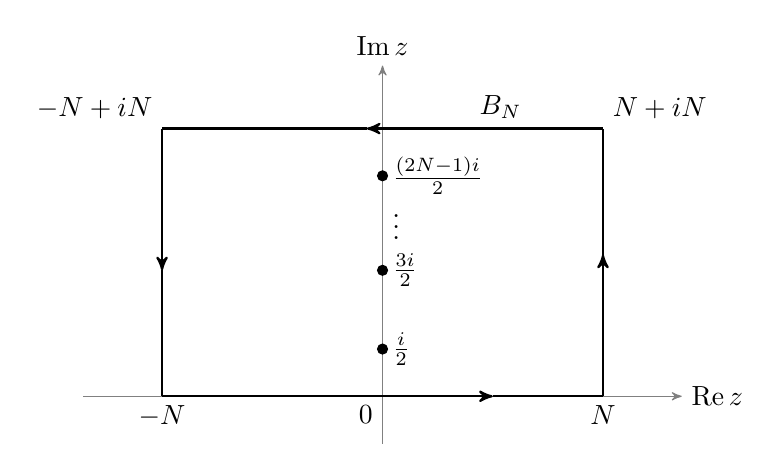
\begin{tikzpicture}
\draw[->,>=stealth',gray] (-3.8,0) -- (3.8,0) node[right,black] {$\operatorname{Re} z$};
\draw[->,>=stealth',gray] (0,-0.6) -- (0,4.2) node[above,black] {$\operatorname{Im} z$};
\draw[thick,->,>=stealth'] (-2.8,0) -- (1.4,0);
\draw[thick] (1.4,0) -- (2.8,0);
\draw[thick,->,>=stealth'] (2.8,0) -- (2.8,1.8);
\draw[thick] (2.8,1.8) -- (2.8,3.4);
\draw[thick,->,>=stealth'] (2.8,3.4) -- (-0.2,3.4);
\draw[thick] (-0.2,3.4) -- (-2.8,3.4);
\draw[thick,->,>=stealth'] (-2.8,3.4) -- (-2.8,1.6);
\draw[thick] (-2.8,1.6) -- (-2.8,0);
\filldraw[black] (0,0.6) circle[radius=1.8pt] node[right] {$\frac{i}{2}$}
                 (0,1.6) circle[radius=1.8pt] node[right] {$\frac{3i}{2}$}
                 (0,2.8) circle[radius=1.8pt] node[right] {$\frac{(2N-1)i}{2}$};
\draw (0,2.25) node[right] {$\vdots$}
      (0,0) node[below left] {$0$}
      (2.8,0) node[below] {$N$}
      (-2.8,0) node[below] {$-N$}
      (2.8,3.4) node[above right] {$N+iN$}
      (-2.8,3.4) node[above left] {$-N+iN$}
      (1.5,3.4) node[above] {$B_N$};
\end{tikzpicture}
\end{document}

